\documentclass[CheatSheet]{subfiles}
\begin{document}


\summarystyle
\section{Kinematics}
This section uses the following notation:
\begin{align*}
&p_i^\mu=\pmat{p^0_i\\\vc p_i}\text{~or~}\pmat{E_i\\\vc p_i}~\text{with $E_i=\sqrt{\|\vc p_i\|^2+m_i^2}$ implying on-shell and $p^0_i$ implying general values},\\
&q_i = \|\vc p_i^\mu\|,\quad s_i = p_i^\mu p_{i\mu}, \quad s_{ij}=(p_i+p_j)^2,\quad s_{ijk}=(p_i+p_j+p_k)^2,~~\cdots;
\\&\text{K\"all\'en function}\quad
\Kallen(x,y,z) = x^2+y^2+z^2-2xy-2yz-2zx = (x-y-z)^2-4yz.
\\&\text{LIPS}\quad
\dd\Pi = \ddP{p}\frac{1}{2E_{p}}
       = \frac{\dd p^0\dd^3\vc p}{(2\pi)^4}\diracdeltabar(p^0;E_p)
;\qquad
\diracdeltabar(p^0;E_p)\coloneq\tpdd((p^0)^2-\vnorm{p}^2-m^2)\Theta(p^0),
\\&\phantom{\text{LIPS}}\quad
  \overline{\dd\Pi^{(n)}}(P;p_i,\dots,p_n) \coloneq  {\dd\Pi_1\cdots\dd\Pi_n\,\tpdd[4]\left(P^\mu-\sum p_i^\mu\right)}.
\end{align*}

\paragraph{Decay rate and cross section}  ($\mathcal M$ has a mass dimension of $4-N\w i-N\w f$.)
\begin{lalignat}{2}
\llabel{decay rate (rest frame; $\sqrt{s}=M_0$):}
\dd\Gamma=
\frac{1}{2M_0}\overline{\dd\Pi^{(N\w f)}}~
\Bigl|\mathcal M\left(M_0\to\left\{p_1, p_2,\cdots, p_{N\w f}\right\}\right)\Bigr|^2
\\
\llabel{cross section (Lorentz invariant):}
\dd\sigma =
\frac{1}{4E_AE_B\,v_{\text{M\o l}}}\overline{\dd\Pi^{(N\w f)}}~
\Bigl|\mathcal M\left(k_A,k_B\to\left\{p_1, p_2,\cdots, p_{N\w f}\right\}\right)\Bigr|^2
\\
\llabel{M\o ller parameter:}\notag
 4E_AE_B v_{\text{M\o l}}= 2s\cdot\Kallen[1/2](1,m_A^2/s,m_B^2/s).
\end{lalignat}


\paragraph{Mandelstam variables} For $(k_A,k_B)\to(p_1,p_2)$ collision,
\begin{alignat*}{3}
 &s = (k_A+k_B)^2 = (p_1+p_2)^2\qquad
 &&(k_A-k_B)^2 =  2(m_A^2+m_B^2)-s\qquad
 &&k_A\cdot k_B = (s-m_A^2-m_B^2)/2\\
 &t = (p_1-k_A)^2 = (p_2-k_B)^2
 &&(p_1-p_2)^2 = 2(m_1^2 + m_2^2) - s
 && p_1\cdot p_2 = (s-m_1^2-m_2^2)/2\\
 &u = (p_1-k_B)^2 = (p_2-k_A)^2
 &&&&k_A\cdot p_2 = (m_2^2 + m_A^2 - u)/2\\
 & s+t+u=m_A^2+m_B^2+m_1^2+m_2^2
 &&&&k_A\cdot p_1 = (m_1^2 + m_A^2 - t)/2
\end{alignat*}

\paragraph{Two-body final state in the CM frame}
$\displaystyle p_1^\mu+p_2^\mu=\pmat{E_1\\\vc p}+\pmat{E_2\\-\vc p}=\pmat{\sqrt s\\\vc 0}$
with $\vc p$ directing to $\Omega=(\theta,\phi)$:
\begin{align}
&\overline{\dd\Pi^{(2)}}\Big|\w{CM}
=\frac{\|\vc p\|}{4\pi\sqrt{s}}\frac{\dd\Omega}{4\pi}
=
\frac{\|\vc p\|}{8\pi \sqrt{s}}\dd\cos\theta
=
\frac{\Kallen[1/2](1,m_1^2/s,m_2^2/s)}{16\pi}\dd\cos\theta
\qquad \Bigl(\text{$\sqrt s = M_0$ or $E\w{CM}$}\Bigr)
\\
\notag&
\|\vc p\|=\frac{\sqrt{s}}{2}\Kallen[1/2]\left(1,\frac{m_1^2}{s},\frac{m_2^2}{s}\right),\quad
 E_1=\frac{s+m_1^2-m_2^2}{2\sqrt{s}},\quad
 E_2=\frac{s-m_1^2+m_2^2}{2\sqrt{s}},\quad
 p_1\cdot p_2 = \frac{s-(m_1^2+m_2^2)}{2}.
\end{align}
Decay rates and 2-to-2 cross sections are
\begin{align}
\dd\Gamma
&\stackrel{\text{CM}}{=}
\frac{\Kallen[1/2](1,m_1^2/s,m_2^2/s)}{32\pi M_0}
  \dd\cos\theta\,|\mathcal M|^2,
&
\dd\sigma
&\stackrel{\text{CM}}{=}
\frac{1}{32\pi s}
  \frac{\Kallen[1/2](1,m_1^2/s,m_2^2/s)}{\Kallen[1/2](1,m_A^2/s,m_B^2/s)}
  \dd\cos\theta\,|\mathcal M|^2
\end{align}


\begin{wrapfigure}[2]{r}{12em}\vspace{-1.5em}
 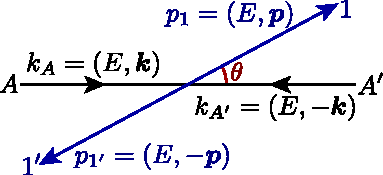
\includegraphics[width=\linewidth,page=1]{figs/collision.pdf}
\end{wrapfigure}

\noindent
For collisions with the same mass $(m_A,m_A)\to (m_1,m_1)$:
\begin{alignat*}{2}
t &= m_A^2+m_1^2 - s/2+2\|\vc k\|\|\vc p\|\cos\theta,\qquad
&\|\vc k\|&={\sqrt{s/4-m_A^2}},\\
u &= m_A^2+m_1^2 - s/2-2\|\vc k\|\|\vc p\|\cos\theta,
&\|\vc p\|&={\sqrt{s/4-m_1^2}}.
\end{alignat*}

\begin{wrapfigure}[2]{r}{12em}\vspace{-2em}
 \includegraphics[width=\linewidth,page=2]{figs/collision.pdf}
\end{wrapfigure}

\noindent
For collisions of massless initial particles $(0,0)\to (m_1,m_2)$:
\begin{alignat*}{2}
 t &= (m_1^2+m_2^2-s)/2+\|\vc p\|\sqrt{s}\cos\theta,\qquad
&\|\vc p\|&=(\sqrt{s}/2)\Kallen[1/2](1,m_1^2/s,m_2^2/s),\\
 u &= (m_1^2+m_2^2-s)/2-\|\vc p\|\sqrt{s}\cos\theta.
\end{alignat*}

\paragraph{Phase-space reduction} With $s'\w{min}=(m_{n+1}+\cdots+m_{n+m})^2$ and $s'\w{max}=(\sqrt{P^2}-m_1-\cdots-m_n)^2$,
\begin{equation}
  \overline{\dd\Pi^{(n+m)}}(P;\,p_1,\dots,p_{n+m})
  =\int_{s'\w{min}}^{s'\w{max}}\frac{\dd s'}{2\pi}
  \,\overline{\dd\Pi^{(n+1)}}(P;\,p',p_{1},\dots,p_{n})
  \,\overline{\dd\Pi^{(m)}}(p';\,p_{n+1},\dots,p_{n+m}),
  \label{eq:psreduction}
\end{equation}
where the two LIPSes are to be evaluated with a constraint $p'^\mu p'_\mu=s'$.

\paragraph{Three-body final state} Mandelstam-like variables can be defined, for $P\to(p_1,p_2,p_3)$, as
\begin{equation*}
s_{ij}=(p_i+p_j)^2;\quad t_{0i}=(P-p_i)^2=s_{jk};\quad s_{12}+s_{23}+s_{31}=P^2+p_1^2+p_2^2+p_3^2.
\end{equation*}
For spherically-symmetric processes, the phase-space integral is reduced to, at the center-of-mass frame,
\begin{align}
\int\overline{\dd\Pi^3}_{\text{sph.\ sym.}}&(\sqrt{s}, \vc 0)
=\frac{1}{128\pi^3}\frac{1}{s}
\int_{(m_2+m_3)^2}^{(\sqrt{s}-m_1)^2}\dd s_{23}\int\dd s_{13};
\\ (s_{13})^{\text{max}}_{\text{min}} &=
\frac{(s+m_3^2-m_1^2-m_2^2)^2}{4s_{23}}
-\frac{1}{4s_{23}}
\left[\Kallen[1/2](s,m_1^2,s_{23})\mp\Kallen[1/2](s_{23},m_2^2,m_3^2)\right]^2
\notag\\&=(E_1^*+E_3^*)^2-\left(\sqrt{E_1^{*2}-m_1^2}\mp\sqrt{E_3^{*2}-m_3^2}\right)^2,
\quad
\end{align}
where 
$E_1^*=\frac{s-s_{23}-m_1^2}{2\sqrt{s_{23}}}$, and
$E_3^*=\frac{s_{23}-m_2^2+m_3^2}{2\sqrt{s_{23}}}$.

\newpage
\detailstyle
\subsection{Fundamentals}

Lorentz-invariant phase space:
\begin{align}
  \dd\Pi
   = \ddP{p}\frac{1}{2E_{p}}
   = \ddP{p}\frac{1}{2\sqrt{m^2+\|\vc p\|^2}}
   = \frac{\dd p_0\dd^3\vc p}{(2\pi)^4}2\pi\diracdelta(p_0^2-\|\vc p\|^2-m^2)\Theta(p^0)
   \equiv \frac{\dd p_0\dd^3\vc p}{(2\pi)^4}\diracdeltabar(p_0;E_p)
\end{align}
K\"all\'en function:
\begin{align*}
&\Kallen(x,y,z)
= x^2+y^2+z^2-2xy-2yz-2zx
= (x-y-z)^2-4yz;
\\
&
\Kallen(1;\alpha_1^2,\alpha_2^2)
= (1-(\alpha_1+\alpha_2)^2)(1-(\alpha_1-\alpha_2)^2)
= (1+\alpha_1+\alpha_2)(1-\alpha_1-\alpha_2)(1+\alpha_1-\alpha_2)(1-\alpha_1+\alpha_2).
\end{align*}
\begin{alignat*}{2}
&s\Kallen[1/2]\left(1,\frac{m_1^2}{s}, \frac{m_2^2}{s}\right) = \Kallen[1/2]\left(s,m_1^2, m_2^2\right);&
\qquad
&\Kallen[1/2]\left(1,\frac{m^2}{s},\frac{m^2}{s}\right)
= \sqrt{1-\frac{4 m^2}{s}},\\
&\Kallen[1/2]\left(1,\frac{m_1^2}{s},\frac{m_2^2}{s}\right)
= \sqrt{1-\frac{2 (m_1^2+m_2^2)}{s}+\frac{(m_1^2-m_2^2)^2}{s^2}},&
&\Kallen[1/2]\left(1,\frac{m_1^2}{s},0\right)
= \frac{s-m_1^2}{s}.
\end{alignat*}

\paragraph{On-shell particles}
The following equations hold for momenta $p_i^\mu$ with $p_i^\mu p_{i\mu}=m_i^2\ge 0$ and $p_i^0\ge 0$:
\begin{alignat}{2}\begin{split}
&(p_1+p_2+\cdots+p_n)^2\ge(m_1+m_2+\cdots+m_n)^2,\\
&(p_1-p_2-\cdots-p_n)^2\le(m_1-m_2-\cdots-m_n)^2.
\end{split}\label{eq:onshell-limit}
\end{alignat}


\subsection{Decay rate and Cross section}\label{sec:xs}
As
$\braket{\text{out}|\text{in}}=(2\pi)^4\diracdelta[4](p\w i-p\w f)\ii\mathcal M$
(for $\text{in}\neq\text{out}$) and $\braket{\vc p|\vc p}=2E_{\vc p}(2\pi)^3\diracdelta[3](\vc 0)=2E_\vc {p}V$ for one-particle state,
\begin{equation}
 \frac{N\w{ev}}{\prod\w{in} N\w{particle}}
= \int\dd\Pi^{\mathrm{out}}\frac{\left|\braket{\text{out}|\text{in}}\right|^2}{\braket{\text{in}|\text{in}}}
= \int\dd\Pi^{\mathrm{out}}\frac{(2\pi)^8|\mathcal M|^2}{\prod\w{in}(2E)V}
\frac{VT}{(2\pi)^4}\diracdelta[4](p\w i-p\w f)
  = VT\int\overline{\dd\Pi^{(N\w f)}}\frac{|\mathcal M|^2}{\prod\w{in}(2E)V}.
\end{equation}
Therefore, decay rate (at the rest frame) is given by
\begin{equation}
 \dd\Gamma
\coloneq  \frac{1}{T}\frac{\dd N\w{ev}}{N\w{particle}}
 = \frac{1}{T}VT\overline{\dd\Pi^{(N\w f)}}\frac{|\mathcal M|^2}{(2E)V}
 = \frac{1}{2M_0}\overline{\dd\Pi^{(N\w f)}}{|\mathcal M|^2}.
\end{equation}
We also define Lorentz-invariant cross section $\sigma$ by $N\w{ev}\eqcolon(n_A v_{\text{M\o l}}T\sigma)N_B=(n_A v_{\text{M\o l}}T\sigma)(n_B V)$ with
number density $n$, or
\begin{equation}
\dd\sigma\coloneq \frac{\dd N\w{ev}}{n_A v_{\text{M\o l}}TN_B}
=
\frac{V}{v_{\text{M\o l}}T}
VT\overline{\dd\Pi^{(N\w f)}}\frac{|\mathcal M|^2}{2E_A2E_BV^2}
=
\frac{1}{2E_A2E_B\,v_{\text{M\o l}}}
\overline{\dd\Pi^{(N\w f)}}|\mathcal M|^2,
\end{equation}
where the M\o ller parameter $v_{\text{M\o l}}$ is equal to $v^{\mathrm{NR}}\w{rel}=\|\vc v_A-\vc v_B\|$ if $\vc v_A\parallel\vc v_B$ (cf.~Ref.~\cite{Cannoni:2016hro}).
Generally,
\begin{equation}
  v_{\text{M\o l}}\coloneq 
 \frac{\sqrt{(p_A\cdot p_B)^2-m_A^2m_B^2}}{E_AE_B}
=\frac{\sqrt{\Kallen(s,m_A^2,m_B^2)}}{2E_AE_B}
=\frac{p_A\cdot p_B}{E_A E_B}v\w{rel}
=({1-\vc v_A\cdot\vc v_B})v\w{rel},
\end{equation}
where $v\w{rel}$ is the actual relative velocity
\begin{equation}
  v\w{rel}
=\sqrt{1-\frac{(1-v_A^2)(1-v_B^2)}{1-(\vc v_A\cdot\vc v_B)^2}}
=\frac{\sqrt{\|\vc v_A-\vc v_B\|^2-\|\vc v_A\times\vc v_B\|^2}}{1-\vc v_A\cdot\vc v_B} =\frac{\Kallen[1/2](s,m_A^2,m_B^2)}{s-(m_A^2+m_B^2)}\neq v^{\mathrm{NR}}\w{rel}.
\end{equation}
(Note that $p_A\cdot p_B/E_AE_B=1$ if $\vc p_A=0$ or $\vc p_B=0$. Also, Each of $v\w{rel}$, $VT$, and $E_AE_Bv_{\text{M\o l}}$ is Lorentz invariant.)



\subsection{Two-body phase space}
Since any Lorentz-invariant function $f(p_1^\mu,p_2^\mu)$ can be written in terms of $q_1$, $q_2$, and $\cos\theta_{12}$, it is convenient to evaluate
\begin{equation}
 \dd\Pi_1\dd\Pi_2
=
\ddP{p_1}\ddP{p_2}\frac{1}{2E_12E_2}
=
\frac{4\pi q_1^2\,\dd q_1\,\cdot 2\pi q_2^2\,\dd q_2\,\dd\cos\theta_{12}}{(2\pi)^6}
\frac{1}{2E_12E_2}
=
\frac{\dd E_+\dd E_- \dd s}{128\pi^4}
\end{equation}
with the replacement of the variables
\begin{align*}
& E_\pm = E_1\pm E_2,
\qquad
s=(p_1+p_2)^2=m_1^2 + m_2^2 + 2E_1E_2 - 2q_1 q_2\cos\theta_{12};\\
&
\left|\frac{\dd(E_+,E_-,s)}{\dd(q_1, q_2, \cos\theta_{12})}\right|=\frac{4q_1^2q_2^2}{E_1E_2},
\qquad
\left|\frac{\dd(E_1,E_2,s)}{\dd(q_1, q_2, \cos\theta_{12})}\right|=\frac{2q_1^2q_2^2}{E_1E_2}.
\end{align*}
Therefore, the two-body phase space integral (without momentum conservation) is given by
\begin{equation}
 \int\dd\Pi_1\dd\Pi_2
=
\frac{1}{128\pi^4}
\int_{(m_1+m_2)^2}^\infty\dd s
\int_{\sqrt{s}}^\infty\dd E_+
\int\w{min}^{\mathrm{max}}\dd E_-,
\end{equation}
where the boundary of $E_-$ is given by
\begin{align*}
 &\cos\theta_{12}=\frac{E_+^2-E_-^2+2 \left(m_1^2+m_2^2-s\right)}{\sqrt{(E_++E_-)^2-4 m_1^2}\sqrt{(E_+-E_-)^2-4 m_2^2}} \in [-1,1]\\
 &\therefore\quad
\left|E_- - \frac{m_1^2-m_2^2}{s}E_+\right| 
\le
\sqrt{E_+^2-s}\cdot\Kallen[1/2]\left(1;\frac{m_1^2}{s},\frac{m_2^2}{s}\right).
\end{align*}

\paragraph{With momentum conservation}
Assume the total momentum is fixed by $P^\mu=(E_0, \vc P_0)$, where $S_0=E_0^2-Q_0^2>0$, as
\begin{equation}
 \overline{\dd\Pi^{(2)}}\times I
   = \dd\Pi_1\dd\Pi_2\,\tpdd[4](P^\mu-p_1^\mu-p_2^\mu)\times I
   =\frac{1}{(2\pi)^2}\frac{\dd^3{\vc p_1}}{2E_1}\frac{\dd^3{\vc p_2}}{2E_2}\diracdelta[4](P^\mu-p_1^\mu-p_2^\mu)\times I
\end{equation}
with $I$ being the integrand. Here, $S_0>0$ and $p^\mu_i p_{i\mu}\ge 0$ are assumed.\footnote{%
Here, $p_1^\mu$ and $p_2^\mu$ are primarily the four momenta of on-shell particles, but we can generalize the discussion to any four momenta with $p_i^\mu p_{i\mu}\ge 0$, such as the sum of two or more momenta of on-shell particles.}
It is then evaluated by
\begin{align}
 \overline{\dd\Pi^{(2)}}\times I
  &= \frac{1}{(2\pi)^2}\frac{\dd^3{\vc p_1}}{2E_1}{\dd^4 p_2^\mu}
  \diracdelta((p_2^0)^2-q_2^2-m_2^2)\Theta(p_2^0)
  \diracdelta[4](P^\mu-p_1^\mu-p_2^\mu)\times I
  \\&=
   \frac{1}{(2\pi)^2}\frac{\dd^3{\vc p_1}}{2E_1}
  \diracdelta((E_0-E_1)^2-\|\vc P_0-\vc p_1\|^2-m_2^2)\Theta(E_0-E_1)\times I
  \\&=
   \frac{1}{(2\pi)^2}\frac{\dd^3{\vc p_1}}{2E_1}
  \diracdelta(S_0-2E_0E_1+2\vc P_0\cdot\vc p_1+m_1^2-m_2^2)\Theta(E_0-E_1)\times I
  \\&=
   \frac{q_1\dd E_1\dd\cos\theta\dd\phi}{8\pi^2}
  \diracdelta(S_0-2E_0E_1+2Q_0q_1\cos\theta+m_1^2-m_2^2)\Theta(E_0-E_1)\times I~\Big|_{q_1=(E_1^2-m_1^2)^{1/2}}.
\end{align}
The following variables are of use, which physically means the energy and momentum of the particles in their center-of-mass frame:
\begin{equation}
  \mathcal E_1=\frac{S_0+m_1^2-m_2^2}{2\sqrt{S_0}},\qquad
  \mathcal E_2=\frac{S_0-m_1^2+m_2^2}{2\sqrt{S_0}},\qquad
  \phi=\frac{\sqrt S_0}{2}\Kallen[1/2]\left(1,\frac{m_1^2}{S_0},\frac{m_2^2}{S_0}\right).
\end{equation}
Here,  $\mathcal E_i^2-\phi_i^2=m_i^2$, $(\mathcal E_1+\mathcal E_2)^2=S_0$, and $E_0\ge \sqrt{S_0}\ge \mathcal E_i\ge m_i$. Then
\begin{align}
 \overline{\dd\Pi^{(2)}}\times I
  &=
   \frac{q_1\dd E_1\dd\cos\theta\dd\phi}{8\pi^2}
  \diracdelta(2\sqrt{S_0}\mathcal E_1-2E_0E_1+2Q_0q_1\cos\theta)\Theta(E_0-E_1)\times I~\Big|_{q_1=(E_1^2-m_1^2)^{1/2}}.
\end{align}


Here, notice that, if the integrand $I$ is a Lorentz scalar, the result is also a Lorentz scalar and independent under Lorentz transformation, so we can set $\vc P_0=\vc 0$. Explicitly, if the integrand $I$ is a constant,
\begin{equation}
 \overline{\dd\Pi^{(2)}}\Big|_{\vc P_0=\vc 0}
  =
   \frac{(E_1^2-m_1^2)^{1/2}\dd E_1}{2\pi}
  \diracdelta(2\sqrt{S_0}\mathcal E_1-2E_0E_1)\Theta(E_0-E_1)
  =
   \frac{\phi}{4\pi\sqrt{S_0}}.
\end{equation}
However, we can proceed with general $\vc P_0$, which is useful to verify the Lorentz invariance but also for general $I$:
\begin{align}
 \overline{\dd\Pi^{(2)}}
  &= \frac{\dd E_1\dd\cos\theta\dd\phi}{16\pi^2 Q_0}
  \diracdelta\left(\cos\theta-\frac{E_0E_1-\sqrt{S_0}\mathcal E_1}{Q_0(E_1^2-m_1^2)^{1/2}}\right)\Theta(E_0-E_1)
\\&=
   \frac{1}{8\pi Q_0}\int_{m_1}^{E_0}{\dd E_1}\,
  \Theta\left(-1\le c(E_1)\le1\right);\qquad
  c(E_1)\coloneq \frac{E_0E_1-\sqrt{S_0}\mathcal E_1}{Q_0(E_1^2-m_1^2)^{1/2}}.
\end{align}
Here, $|c(x)|=1$ has two solutions $x_\pm=(E_0\mathcal E_1\pm Q_0\phi)/\sqrt{S_0}$, which correspond to\footnote{%
  Notice that $E_{\text{1; min}}^2-m_1^2=(Q_0\mathcal E_1-E_0\phi)^2/S_0>0$
  and
$E_0-E_{\text{1; max}}=(E_0^2m_2^2+S_0\phi^2)/(\sqrt{S_0}(E_0\mathcal E_2+Q_0\phi))>0$.
}
\begin{equation}
  E_{\text{1; max}}=\frac{E_0\mathcal E_1+Q_0\phi}{\sqrt {S_0}},\quad
  q_{\text{1; max}}=\frac{Q_0\mathcal E_1+E_0\phi}{\sqrt{S_0}};\qquad
  E_{\text{1; min}}=\frac{E_0\mathcal E_1-Q_0\phi}{\sqrt {S_0}},\quad
  q_{\text{1; min}}=\frac{\left|Q_0\mathcal E_1-E_0\phi\right|}{\sqrt{S_0}}.
\end{equation}
Meanwhile, $c'(x)$ becomes zero at $x_0=(E_0 m_1^2)/(\sqrt {S_0}E_1)$, where $\sign(x_0-x_-)=\sign(Q_0 \mathcal E_1-E_0\phi)$.
Therefore,
\begin{itemize}
  \item if $Q_0 \mathcal E_1<E_0\phi$, $c(x)$ is monotonically increasing from $c(x_-)=-1$ to $c(x_+)=+1$.
  \item if $Q_0 \mathcal E_1>E_0\phi$, $c(x)$ has a minimum $\displaystyle c(x_0)=\frac{\sqrt{Q_0^2\mathcal E_1^2-E_0^2\phi^2}}{Q_0m_1}$ and $c(x_-)=c(x_+)=+1$.
\end{itemize}
In either cases, the Heaviside function becomes unity between $E_{\text{1; min}}$ and $E_{\text{1; max}}$, i.e.,
\begin{equation}
 \overline{\dd\Pi^{(2)}}
= \frac{1}{8\pi Q_0}\int_{m_1}^{E_0}{\dd E_1}\,
  \Theta\left(-1\le c(E_1)\le1\right)
= \frac{1}{8\pi Q_0}\int_{E_{\text{1; min}}}^{E_{\text{1; max}}}{\dd E_1}
= \frac{\phi}{4\pi \sqrt{S_0}}.
\end{equation}
This discussion can be applied to general integrands. Schematically, we can evaluate the integral as
\begin{align}
 \overline{\dd\Pi^{(2)}}\times I
  &=\frac{1}{8\pi Q_0}
   \int_{m_1}^{E^0}{\dd E_1}{\dd\cos\theta}\cdot
  \diracdelta\left(\cos\theta-\frac{E_0E_1-\sqrt{S_0}\mathcal E_1}{Q_0(E_1^2-m_1^2)^{1/2}}\right)
  \times \left(\frac{\dd\phi}{2\pi} I\right)~\Bigg|_{\text{$p_2^\mu$ and $q_1$ being fixed}}
  \\
  &=\frac{1}{8\pi Q_0}
   \int_{E_{\text{1; min}}}^{E_{\text{1; max}}}{\dd E_1}
  \times \left(\frac{\dd\phi}{2\pi} I\right)~\Bigg|_{\cos\theta=c(E_1);~~\text{$p_2^\mu$ and $q_1$ being fixed}}
\label{eq:twobody-direct}
\end{align}
for most cases.




\subsection{More than two bodies}
The phase-space reduction formula \eqref{eq:psreduction} is proved by, with $p_{a,\dots,b}=\sum_{i=a}^b p_i$, (cf.~Ref.~\cite{Hitoshi233B})
\begin{align*}
  \overline{\dd\Pi^{(n+m)}}%(P;\,p_1,\dots,p_{n+m})
  &=\left[
    \ddP{p'}\frac{\dd p'^0}{2\pi}\tpdd[4]\left(p'^\mu-p_{1,\dots,n}^\mu\right)
  \right]
  \dd\Pi_1\cdots\dd\Pi_{n+m}\,\tpdd[4]\left(P^\mu-p_{1,\dots,n+m}^\mu\right)
\\ &=    \left[
    \overline{\dd\Pi^{(n)}}(p';\,p_1,\dots,p_n)\,
    \overline{\dd\Pi^{(m+1)}}(P;\,p',p_{n+1},\dots,p_{n+m})\,
  \right]
    \frac{\dd p'^0}{2\pi}(2p'^0)
\\ &=    \left[
    \overline{\dd\Pi^{(n)}}(p';\,p_1,\dots,p_n)\,
    \overline{\dd\Pi^{(m+1)}}(P;\,p',p_{n+1},\dots,p_{n+m})\,
  \right]_{p'^\mu p'_\mu=s'\text{~:~fixed}}
    \frac{\dd s'}{2\pi},
\end{align*}
where the range of $\dd s'$ is limited to, due to Eq.~\eqref{eq:onshell-limit},
\[
(m_1+m_2+\cdots+m_n)^2\le s'\le (\sqrt{P^2}-m_{n+1}-\cdots-m_{n+m})^2.
\]


For a constant integrand and massless particles, the phase-space integral is obtained by, since we can set $P^\mu=\spmat{\sqrt{S_0}\\\vc 0}$,
\begin{align}
\int1\,\overline{\dd\Pi^{(n)}}(S_0)
&= \frac{\dd s'}{2\pi}
  \overline{\dd\Pi^{(2)}}(P_0;\,p',p_{n})\,
  \overline{\dd\Pi^{(n-1)}}(p';\,p_1,\dots,p_{n-1})
= \int_0^{S_0}\frac{\dd s'}{2\pi}
\frac{\Kallen[1/2](1,s'/S_0,0)}{8\pi}
  (a_{n-1}s'^{n-3})
\notag\\&
= \frac{a_{n-1}}{(4\pi)^2(n-1)(n-2)}S_0^{n-2}
\qquad\therefore\quad
\int1\,\overline{\dd\Pi^{(n)}}=
  \frac{1}{2(4\pi)^{2n-3}}\frac{S_0^{n-2}}{(n-1)!(n-2)!}
\end{align}
where the fact is used that $\overline{\dd\Pi^{(n)}}(s)=a_n\times s^{n-2}$ with $a_n$ being a constant.

\paragraph{Three-body: spherically-symmetric cases}
For spherically-symmetric (as well as Lorentz invariant) integrand, we evaluate the three-body phase space at the center-of-mass frame as
\begin{align}
  \overline{\dd\Pi^{(3)}}_{\text{sph-sym}}
  &=\frac{\dd s_{23}}{2\pi}
  \overline{\dd\Pi^{(2)}}(P_0;\,p_1,p_{23})
  \overline{\dd\Pi^{(2)}}(p_{23};\,p_2,p_3)
\\
  &=\frac{\dd s_{23}}{2\pi}\cdot
   \frac{q_1\dd E_1\dd\cos\theta\dd\phi}{8\pi^2}
  \diracdelta(2\sqrt{S_0}\mathcal E_1-2E_0E_1)\Theta(E_0-E_1)\cdot
  \frac{1}{8\pi q_{23}}\dd E_3\frac{\dd\phi_{2,3}}{2\pi}
\\
  &=\frac{\dd s_{23}}{2\pi}\cdot
   \frac{q_1\dd E_1}{4\pi \sqrt{S_0}}
  \diracdelta(E_1-\mathcal E_1)\cdot
  \frac{1}{8\pi q_{23}}\dd E_3,
\end{align}
where angular integrals are carried out naively and $\mathcal E_1=(S_0+m_1^2-s_{23})/2\sqrt{S_0}$. As $q_1=q_{23}$ and $s_{12}=S_0+m_3^2-2E_3\sqrt{S_0}$,
\begin{align}
  \overline{\dd\Pi^{(3)}}_{\text{sph-sym}}
  &=\frac{\dd s_{23}\dd E_3}{64\pi^3\sqrt{S_0}}
  =\frac{1}{128\pi^3S_0}
\int_{(m_2+m_3)^2}^{(\sqrt{s}-m_1)^2}\dd s_{23}\int\dd s_{12},
\end{align}
which is equal to the PDG-Eq.~(47.23)\cite{PDG2018}. The second integral is to be evaluated between
\begin{align}
&(E_3)_{\text{max}}^{\text{min}} =
\frac{E_{23}\mathcal E_{3;23}\mp q_{23}\phi_{23}}{\sqrt{s_{23}}}
=
\frac{(S_0+s_{23}-m_1^2)(s_{23}-m_2^2+m_3^2)\mp\Kallen[1/2](S_0,m_1^2,m_2^2) \Kallen[1/2](s_{23},m_2^2,m_3^2)}{4\sqrt{S_0}s_{23}},
\\&\text{i.e.,}\quad
(s_{12})_{\text{min}}^{\text{max}} =
\frac{(S_0+m_2^2-m_1^2-m_3^2)^2-\left[
\Kallen[1/2](S_0,m_1^2,m_2^2) \mp \Kallen[1/2](s_{23},m_2^2,m_3^2)
\right]^2}{4s_{23}}.
\end{align}


\subsection{Two-body decay of boosted particles}
A particle with $(P, \Theta, \Phi; M)$ decaying to two particles; at the CM frame the momenta of the decay products are characterized by $\vc q=(q,\theta,\phi)$ with $q=(M_0/2)\Kallen[1/2](1,m_1^2/M_0^2,m_2^2/M_0^2)$. Their lab-frame momenta are given by
\begin{align}
 P &=
\begin{pmatrix}
  E_0\\
 {P_0} \si\Theta \co\Phi \\
 {P_0} \si\Theta \si\Phi \\
 {P_0} \co\Theta \\
\end{pmatrix},&
 p_1&=
\begin{pmatrix}
  ({E_0 \mathcal{E}_1+P_0 q \co\theta})/{M_0} \\
 q \co\Theta \co\Phi \si\theta \co\phi - q \si\Phi \si\theta \si\phi + r_1 \si\Theta \co\Phi \\
 q \co\Theta \si\Phi \si\theta \co\phi + q \co\Phi \si\theta \si\phi   + r_1 \si\Theta \si\Phi \\
 -q \si\Theta \si\theta \co\phi + r_1 \co\Theta\\
\end{pmatrix},&
p_2&=
\begin{pmatrix}
  ({E_0 \mathcal{E}_2-P_0 q \co\theta})/{M_0} \\
 -q \co\Theta \co\Phi \si\theta \co\phi + q \si\Phi \si\theta \si\phi + r_2 \si\Theta \co\Phi \\
 -q \co\Theta \si\Phi \si\theta \co\phi - q \co\Phi \si\theta \si\phi + r_2 \si\Theta\si\Phi  \\
  q \si\Theta \si\theta \co\phi+r_2 \co\Theta \\
\end{pmatrix}
\end{align}
with $r_1=(P_0\mathcal{E}_1+E_0q\co\theta)/M_0$, $r_2=(P_0\mathcal{E}_2-E_0q\co\theta)$, and $\mathcal{E}_i=\sqrt{m_i^2+q^2}$.


\end{document}
